% Dokumentklassen sættes til memoir
\documentclass[a4paper,11pt,article,oneside,final]{memoir}

\usepackage[utf8]{inputenc}
\usepackage[T1]{fontenc}
\usepackage[english]{babel}

% Matematiske symboler og fede tegn i ligninger
\usepackage{amsmath, amssymb, bm, mathtools, float}
\usepackage{longtable}

% Tabeller og søjler
\usepackage{array, booktabs, dcolumn}
\newcolumntype{d}[1]{D{,}{,}{#1}} % Justering under komma

% Figurer
\usepackage{graphicx, caption, subfig}
\captionsetup{font=small,labelfont=bf}

% PDF include
\usepackage{pdfpages}

% Bibtex
\usepackage{natbib}

% Algorithmer
% \usepackage{algorithm}
% \usepackage{algorithmic}
\usepackage{listings}
\usepackage{lscape}

\usepackage{hyperref}
\hypersetup{
    colorlinks,
    citecolor=black,
    filecolor=black,
    linkcolor=black,
    urlcolor=black
}

\pagestyle{companion}
\title{Course Name}
\author{
		{\noindent\HUGE\bfseries Project Name} \\ \\ \\
		%		Peter Urbak, 20081130 \\
		%		Jakob Schultz-Nielsen, 20061951 \\
		%		Morten Rasmussen, 20060914 \\ 
		%		Lasse Højgaard, 20080848 \\
		Frederik Mogensen, 20080923 \\
}
\date{31. maj 2011}

\begin{document}
	\sloppy
	\maketitle

	\newpage
	\tableofcontents
	\cleardoublepage

	    \begin{frame}[t]
	\frametitle{Headline - Very Serious}
	One item
	\begin{itemize}
		\item Here it is.
	\end{itemize}
	\pause
	\vspace{0.5cm}
	Two items
	\begin{itemize}
		\item Item 1. \pause
		\item Item 2.
		\item Item 3.
	\end{itemize}
	\note[item] {Not actually serious}
	\note[item] {
	Venn Diagrams
	\\
		\begin{figure}[h]
			\centering
			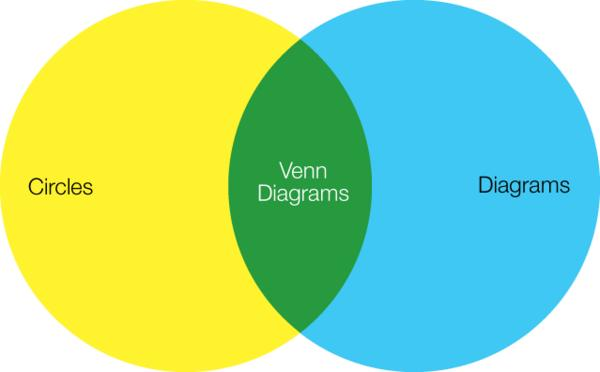
\includegraphics[height=\textheight/2]{img/venndiagram.jpeg}
			\label{fig:venndiagram-meta}
		\end{figure}
	}
\end{frame}

\begin{frame}[t]
	\frametitle{Range query searching}
	\begin{block}{S1. [Search subtrees.]}
		 Check each entry $E$ to determine whether the MBR overlaps $q$.
		 For all overlapping entries, invoke \emph{Search} on the tree whose
		 root is pointed to by $E.p$
	\end{block}

	\begin{block}{S2. [Search leaf node.]}
		Check all entries $E$ to determine whether the MBR overlaps $q$.
		If so, $E$ is a qualifying record
	\end{block}
\end{frame}




% 	\newpage
% 	\input{content/bilag.tex}
\bibliographystyle{plain}
\bibliography{references}
\end{document}

